\chapter{Reinforcement Learning}
\label{ch:rl}
\thispagestyle{empty}

When we think about the nature of learning, the first thing that probably occurs to us is learning by examples, namely, learning from some interactions with the environment that builds up our experience. Since we were children, we started interacting with the environment: we take some action, we see its consequence and we repeat until we accomplish a goal (e.g. we start moving the feet and learn how to walk). 


Reinforcement Learning (RL) is a field of Machine Learning that closely resembles how living beings learn in nature. In this work we will explore the computational approach to learning from interaction, by considering a simplified yet powerful mathematical model. The final result will be a function that maps actions to each state, that tells us what to do, so as to maximize a reward signal. This reward signal is intended to give insights about \textit{what} is the goal to pursue but not \textit{how}. The learner is not told which actions to take, but rather he has to discover which actions are more valuable via trial and error, from experience \\
This is not a trivial task, since actions can potentially have long-term effects. As a matter of facts, an action affects the following state, from where another action can lead to another state and so on, generating a sequence of causally related events. Delayed rewards and trial and error search are the two most important aspects of reinforcement learning, that makes this problem both difficult and intriguing.

We will formalize the problem of reinforcement learning using a model taken from dynamical systems theory called Markov decision process. This model is able to capture the interactions between the agent and the environment and will be described in details in \Cref{sec:mdp}. Next, three general methods to solve a MDP are presented in \Cref{sec:solve-mdp}: policy iteration, value iteration and policy search. We will briefly describe the former two methods enough to introduce a policy search method called Policy Gradient, that is of main interest in this work. Policy Gradient method will then be described in details in \Cref{sec:policy-gradient}, including some aspects about gradient approximation, baselines and other more advanced refinements.








\section{Markov Decision Processes}
\label{sec:mdp}
In this section we will formalize the problem of reinforcement learning by defining a mathematical model called Markov decision process.\\
The main aspects that we want to capture are the interactions between an agent and the environment over time. A learning agent must be able to sense the state of its environment and take some actions, while the environment itself receives the actions from the agent and reacts by changing the state and giving feedbacks to the agent to complete a cycle.
The agent must also have a goal that is related to a state of the environment.\\
Markov decision processes are intended to include just these three aspects -- sensation, action and goal -- in their simplest possible forms without trivializing any of them.

\begin{definition}
A Markov Decision Process (MDP) is a tuple $\left\langle \sspace, \aspace, \tfunc, \rfunc, \gamma, \mu \right\rangle$  where:
\begin{itemize}
\item $\sspace$ is the set of possible \textbf{states}
\item $\aspace$ is the set of possible \textbf{actions}
\item $\tfunc : \sspace \times \aspace \rightarrow \Delta (\sspace)$ is the \textbf{transition function} that, given the current state and current action, outputs a probability distribution over the next state.
\item $\rfunc : \sspace \times \aspace \rightarrow \mathbb{R}$ is the \textbf{reward function} that maps a scalar reward to every state-action pair
\item $\gamma$ is the \textbf{discount factor}
\item $\mu : \Delta ( \sspace )$ is a probability distribution over the \textbf{initial state}. 
\end{itemize}
\end{definition}

Note that the above definition of Markov Decision Process encodes two important properties:
\begin{itemize}
\item[-] Stationarity: the transition function $\tfunc$ does not change over time.
\item[-] Markov property: the transition function $\tfunc$ only depends on the previous state, not on the entire history.
\end{itemize}
This mathematical model is very general and can be used to model different problems:

\begin{example}[Chess]
The game of chess can be modelled as an MDP with a discrete state space that encodes the position of all the pieces in the checkerboard, a discrete action space encoding all the possible moves of the pieces, deterministic transition function that follows the rules of the game and a possible reward function:
\begin{equation*}
\rfunc(s,a) = \begin{cases}\,\,\,\,\,1 & \textrm{Player wins} \\ -1 & \textrm{Player does not win} \end{cases}
\end{equation*}
\end{example}

\renewcommand\windowpagestuff{\centering 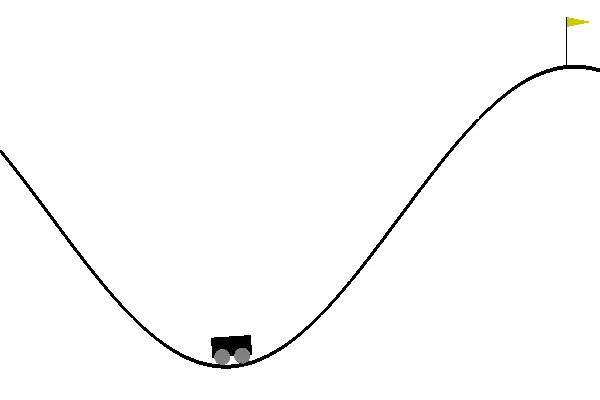
\includegraphics[width=5.5cm]{pictures/mountain_car} \captionof{figure}{Mountain car task}}
\opencutright

\begin{adjustbox}{valign=C,vspace=0bp,minipage={1.0\linewidth}}
\begin{example}[Mountain Car]
\begin{cutout}{0}{7.5cm}{0pt}{12}
A car is placed between two hills and can move left or right. The goal is to reach the top of the right hill, but the engine is not powerful enough to directly climb the hill, so the optimal solution is to gain velocity by first going in the opposite direction. This task can be modelled with a continuous state space $\sspace \in [-2, 2]$, continuous action representing the force applied to the car $\aspace \in [-1, 1]$, deterministic transition function given by physics laws and the following reward function:
\end{cutout}

\begin{equation*}
\rfunc(s,a) = \begin{cases} +100 & \textrm{when } s \geq 1.5 \\ -a^2 & \textrm{otherwise} \end{cases}
\end{equation*}

This problem is particularly difficult for its exploration need: the agent, in fact, must explore very much in order to see the goal, but this comes with a cost associated to the square of the taken action.
\end{example}

\end{adjustbox}


\renewcommand\windowpagestuff{\centering 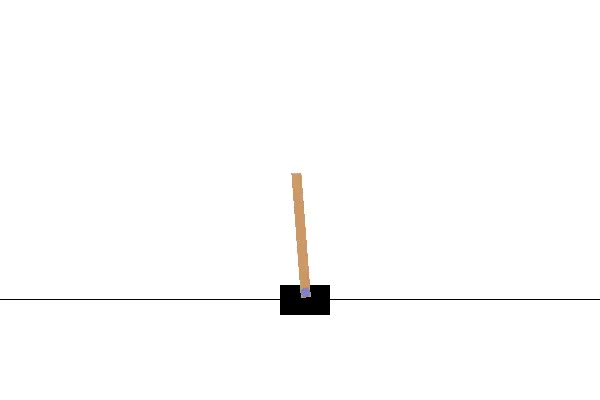
\includegraphics[width=5.5cm]{pictures/cartpole} \captionof{figure}{Cartpole task}}
\opencutleft
\begin{adjustbox}{valign=C,vspace=0bp,minipage={1.0\linewidth}}
\begin{example}[Cartpole]

\begin{cutout}{3}{0pt}{8cm}{13}
A pole is attached to a cart by a joint that is free to rotate. The cart moves along a frictionless track either left or right. The pole starts upright, and the goal is to prevent it from falling over by moving the cart left-right.\\
This task can be modelled with a continuous multidimensional state space $\sspace \in \mathbb{R}^4$. The state features are: the position of the cart $s_0 \in [-2.4, 2.4]$, its velocity $s_1 \in [-\infty, \infty]$, the pole angle $s_2 \in [-\frac{\pi}{2}, \frac{\pi}{2}]$ and its angular velocity $s_3 \in [-\infty, \infty]$. The action space is continuous $\aspace \in [-1, 1]$ and represents the force to be applied on the cart. The transition function is given by physics laws and the reward is $+1$ for every step until the episode ends. An episode ends when a maximum step limit $H$ is reached or when the pole is inclined more than 15 degrees from vertical.


\end{cutout}

\end{example}
\end{adjustbox}

\begin{figure}[t]
\centering
\includegraphics[width=0.9\textwidth]{pictures/mdp_agent_environment}
\caption{Agent-environment loop}
\end{figure}

An agent in a MDP starts from an initial state drawn from the probability distribution $\mu$, $s_0 \sim \mu$. From this state, the agent can interact with the environment by executing an action $a_0 \in \aspace$. The environment receives action $a_0$ and reacts to this stimulus by returning to the agent the next state $s_1$ drawn from the transition function $s_1 \sim \tfunc(s_0, a_0)$ and a scalar reward $r_1 = \rfunc(s_0, a_0)$. From its new observation, the agent can continue the interaction with the environment by choosing another action $a_1$ and so on until it reaches the goal. We define the collected sequence of states, actions and rewards $\tau \sim s_0, a_0, s_1, r_1, a_1, s_2, \ldots$ trajectory. Sometimes we will refer to a trajectory with terms like samples or experience, since these collected informations will be used for the learning procedure.


Intuitively, the agent aims at maximizing the sum of the collected rewards. However this naive sum of rewards do not apply if we consider infinite-horizon MDPs, which is a common setting in the literature. In fact, summing over potentially infinite-length trajectories will cause the cumulative reward to grow indefinitely and lose its original meaning. (e.g. earning +1 at every step will have the same meaning of earning +100 at every step, since over an infinite horizon they will both grow to infinity).\\
For this reason, it is common to consider a generalized version where we apply a discount factor $\gamma$ to the immediate reward and consider the cumulative discounted reward:
\begin{definition}[Cumulative discounted reward]
\begin{equation*}
R = \sum_{t=0}^{\infty} \gamma^t r_t
\end{equation*}
where $\gamma \in [0,1]$ is called discount factor. 
\end{definition}
Note that the naive cumulative reward can be obtained by setting $\gamma=1$, and this is commonly used when the horizon is finite. 

However, the addition of the discount factor has a well-known two-fold meaning: at a first glance, it represents how the agent is interested in future rewards. With $\gamma$ close to $0$, we have a myopic behaviour, where we are only interested in immediate rewards rather than long-term investments. With $\gamma$ close to $1$, instead, we are giving more value to long-term rewards. In the second place, $\gamma$ can also represent the probability that the simulation will continue for one more step. If $\gamma$ is low, we should strive to get as much as we can because we don't have any assurance that we could last one more step.
The discount factor usually depends on the domain and the goal that we want to achieve: a long-term goal will require a value of $\gamma$ close to $1$.


The actual value of the discounted cumulative reward depends on the interaction of the agent over a trajectory. Many factors come into play to influence this objective function, most importantly the behaviour of the agent (e.g. which actions the agent chooses). The way an agent interacts with the environment and hence characterizes its behaviour is defined by the policy function:
\begin{definition}
A policy $\pi: \sspace \rightarrow \Delta (\aspace)$ is a function that for each state $s \in \sspace$ outputs a probability distribution over the actions in $\aspace$. In other words, from state $s$ the agent will choose action $a$ with probability $\pi(a \mid s)$.
\end{definition}

The policy is one of the main ingredients of reinforcement learning, as it is the final result of a reinforcement learning algorithm. The policy tells the agent which actions to choose in every state.
Starting from an initial state $s_0$, the agent will choose action $a_0 \sim \pi(\cdot | s_0)$ drawn from the action distribution induced by the policy in this state. We can see that, given an initial state, a policy completely define all the interaction with the environment, hence we can define its performance or expected return in this way:
\begin{definition}[Performance of a policy $\pi$]
The performance (or expected return) of a policy $\pi$ under initial state distribution $\mu$ is:
\[
J_\mu(\pi) = \EV[a_k \sim \pi, s_0 \sim \mu]{R}
\]
that is, the expected value of the discounted cumulative reward obtained by following the policy $\pi$ starting from an initial state drawn from $\mu$.
\end{definition}
Having defined this new metric, we can easily rank each policy according to its performance: a policy $\pi_1$ is better than a policy $\pi_0$ if $J_\mu(\pi_1) > J_\mu(\pi_0)$. The next step will be to find the policy that scores the highest performance for a given MDP. This is the goal of solving an MDP.

\textbf{Problem formulation:}\quad
To solve a MDP means to find an optimal policy $\pi^*$ that maximizes the average cumulative reward. More formally we want to find $\pi^*$ such that $J_\mu(\pi^*)=\EV[a_k \sim \pi^*, s_0 \sim \mu]{R}$ is maximum.

Summing up, we can define the interaction between an agent and the environment as a sequence of state-action-reward tuples called trajectory. The environment is modelled with a markovian transition function - a function that takes the current state-action pair and outputs a probability distribution over the next state. The Markov property assures that the transition function depends only on the current state and not on the entire history of the interaction. The agent receives a reward for every action it takes and aims at maximizing the discounted cumulative reward. The behaviour of the agent is characterized by the policy function $\pi$, which yields for every state $s$ a probability distribution over the actions $\pi(a|s)$. Every policy can be ranked by its performance or expected reward obtained following the policy from an initial state drawn from $\mu$. A MDP is considered solved when we find an optimal policy $\pi^*$ whose performance value is maximal.

Here we define a new quantity that will be useful later which is the discounted future state distribution. This function calculates the visitation frequency for each state $s\in\sspace$ by starting from $s_0\sim\mu$ and following policy $\pi$. This quantity is defined as follows:
\begin{definition}[Future state distribution]
The (discounted) future state distribution is defined as: 
\[
d_{\mu}^{\pi}(s) = (1-\gamma)\sum_{t=0}^{\infty} \gamma^t Pr(s_t = s)
\]
This quantity identifies the expected state distribution starting from $s_0 \sim \mu$ and following policy $\pi$. 
\end{definition}

Following this definition, we can reformulate the performance of a policy $\pi$ as a function of the state distribution $d_\mu^\pi(s)$.

\begin{definition}[Performance given state distribution]
The performance of a policy $\pi$ given an initial state distribution $\mu$ can be expressed as: 
\begin{equation*}
J_{\mu}(\pi) = \int_{\sspace} d_{\mu}^{\pi}(s) \int_{\aspace} \pi(a \mid s) \rfunc(s,a) \de a \de s
\end{equation*}
\end{definition}


\subsection{Value functions}
So far we have defined what is a MDP and what does it mean to find an optimal policy $\pi*$. In this part we will take the problem under a different perspective by considering the value of each state. The value of a state should not consider only immediate rewards, but should also consider the discounted sum of all the rewards that the agent may get. This idea of including delayed rewards to describe the value of a state is defined by the state-value function:

\begin{definition}[State-value function]
The value of a state $s$ that can be obtained by running policy $\pi$ is given by:
\[
V^{\pi}(s) = \int_{\aspace} \pi(a \mid s) \left( \rfunc(s,a) + \gamma \int_{\sspace} \tfunc(s' \mid s, a) V^{\pi} (s') \de s' \right) \de a
\]
\end{definition}

The state-value function $V^\pi(s)$ encodes the average reward that we will obtain starting from state $s$ and following $\pi$ thereafter. Note that this is a recursive definition as to compute the value of state $s$ we need to compute the values of all the states reachable from $s$ and so on. This definition allows us to give a different way to calculate the performance of a policy based on the value function and initial state distribution
\[
J_\mu(\pi) = \int_{\sspace}\mu(s)V^\pi(s)\de s
\]
The value of the optimal policy $\pi^*$ is called optimal state-value function $V^*(s) = V^{\pi^*}(s)$. The optimal value function is unique, even if multiple optimal policies may exist. We can restate the goal of an RL algorithm as a maximization over the policy space of the state-value function for all states:
\[
\pi^* = \arg\max_{\pi \in \Pi} V^\pi(s),\qquad \forall s \in \sspace
\]
The value function is useful to consider to solve a MDP, however it does not say anything about the actions that brought to that value. Since our main goal is to find an optimal policy, we need a way to assign a value also to the actions. The following statement will define the action-value function:

\begin{definition}[Action-value function]
The action-value function for a policy $\pi$ is defined as follows:
\[
Q^{\pi}(s, a) = \rfunc(s, a) + \gamma \int_{\sspace} \tfunc (s' \mid s, a) \int_{\aspace} \pi(a' \mid s') Q^{\pi} (s', a') \de a' \de s'
\]
\end{definition}

The action-value function defines the value that we can obtain starting from state $s$ and executing action $a$. This function encodes more informations since we can retrieve the state-value function by averaging the action-value function over all actions: $V^\pi(s) = \EV[a\in\aspace]{Q^\pi(s,a)}$. \\
Similarly to the definition of the optimal value function, the optimal action-value function $Q^*$ is defined to be the action-value function of the optimal policy $Q^*(s) = Q^{\pi^*}$. 

The action-value function let us introduce another quantity of particular interest for the algorithms described in \Cref{sec:solve-mdp} called the advantage function. The advantage of action $a$ over policy $\pi$ encodes how much we can gain by performing action $a$ instead of following the policy $\pi$ and is defined as follows:
\begin{definition}[Advantage function]
The advantage function of action $a$ over policy $\pi$ is defined as:
\[
A^{\pi}(s,a) = Q^{\pi}(s,a) - V^{\pi}(s)
\]
\end{definition}

The advantage function can also be used to compare two policies $\pi'$ and $\pi$: for every state $s$ we compute the advantage of selecting an action from $\pi'$ rather than $\pi$. In this case it is called policy advantage function.
\begin{definition}[Policy advantage function]
The advantage of policy $\pi'$ with respect to policy $\pi$ in state $s$ can be computed as:
\[
A_\pi^{\pi'}(s) = \int_{\aspace} \pi'(a|s)A^\pi(s, a) \de a
\]
whose expected value over the states is called expected policy advantage function:
\[
\poladv[\pi,\mu][\pi'] = \int_{\sspace} d_\mu^{\pi}(s)A_\pi^{\pi'}(s) \de s
\]
\end{definition}

Note that the greedy policy is the one that has always non-positive advantage for each state. 


\section{General methods to solve a MDP}
\label{sec:solve-mdp}

In the previous section we have seen that solving a MDP means finding an optimal policy $\pi^*$ with highest performance $J_\mu(\pi)$ which yields the optimal state-value function $V^*(s)$. Before diving into specific methods that aims at solving a MDP, we will proceed to describe some classification for learning algorithm classes.\\
First of all, we have to distinguish between a \textit{target} policy and a \textit{behaviour} policy: the target policy is the output of the algorithm, the one that is intended to solve the MDP. The behaviour policy, instead, is a policy that is used to collect the trajectory samples that will be used for learning. Depending on how the trajectories used to learn the target policy are collected, a learning algorithm can operate on-policy or off-policy:
\begin{itemize}
\item \textbf{On-policy}: the behaviour policy corresponds to the target policy. This means that every collected trajectory is sampled from the current policy. In simpler terms, it means that the agent learns from his own experience.
\item \textbf{Off-policy}: the target policy differs from the behaviour policy. In this case, the agent will learn from 'someone else'. Note that 'someone else' can also mean from itself in a different time-frame.
\end{itemize}

Another difference between the learning algorithms arises when we consider the degree of knowledge about the environment that the agent has:
\begin{itemize}
\item \textbf{Model-based}: the agent has a model of the environment, which can be either exact or approximated. Note that if the agent has an exact model, then the MDP can be solved even without experience.
\item \textbf{Model-free}: the agent has no information about the environment. The only way to learn is by collecting samples from the environment.
\end{itemize}

This concludes our partial taxonomy of RL methods. Of course there are other aspects that are used to classify a RL method, but these are out of scope for this work. We will only consider model-free on-policy methods. This is a common scenario for  control problems where it is possible to collect samples from the environment but it may not be possible to build an exact model of it.\\
The following sections will describe the three main methods that are used to solve a MDP: policy iteration, value iteration and policy search.

\subsection{Policy iteration}
As we have seen in the previous section, the state-value function associates a value to each state of a MDP by considering all the discounted future rewards that can be taken by following a policy $\pi$ from that state. The state-value functions associated to different policies can be used to define an ordering relationship between policies:

\begin{definition}[Policy improvement]
Given two policies $\pi, \pi' \in \Pi$, policy $\pi'$ is better than or equal to ($\succcurlyeq$) policy $\pi$ when the value function of $\pi'$ is greater than or equal to the value function of $\pi$ in all states:
\[
\pi' \succcurlyeq \pi \Longleftrightarrow V^{\pi'}(s) \geq V^{\pi}(s),\quad \forall s \in \sspace
\]
\end{definition}

A policy $pi'\succcurlyeq\pi$ can be found by taking, for each state, the action that yields the highest value. The policy so constructed is called greedy policy and can be found via maximization over actions of the action-value function:
\begin{definition}[Greedy policy]
The greedy policy is the policy that chooses the action that yields the highest value for each state:
\[
\tilde{\pi}(a|s) = \arg\max_{a\in\aspace} Q^{\pi}(s,a), \qquad \forall s \in \sspace
\]
\end{definition}

The greedy policy $\tilde{\pi}$ is an improvement of the policy $\pi$ as it occurs that $\tilde{\pi}\succcurlyeq\pi$. This result is known as the policy improvement theorem~\cite{BELLMAN1958228}. Successive improvements require the evaluation of the newly found policy to obtain its associated action-value function.\\
Policy iteration method~\cite{howard:dp} aims at finding a sequence of policies $\pi^0 \succcurlyeq \pi^1  \succcurlyeq \pi^2 \ldots$ by alternating the improvement and the evaluation of the policy:
\begin{itemize}
\item Policy evaluation: we evaluate the current policy $\pi^k$ on the MDP and we compute the corresponding action-value function $Q^{\pi^k}(s,a)$.
\item Policy improvement: we improve the current policy by computing the greedy policy from the computed action-value function: $\pi^{k+1} \gets greedy\left( Q^{\pi^k} \right)$
\end{itemize}

This algorithm is guaranteed to converge in few iterations to the optimal policy $\pi^*$ when the state-action function $Q(s,a)$ can be computed exactly \cite{10.2307/3689239}, \cite{6796861}, \cite{Tsitsiklis:2003:COP:944919.944922}.\\
This approach, though, suffer from these limitations:
\begin{itemize}
\item In practical scenarios it is not possible to exactly evaluate the action-value function $Q^\pi(s,a)$ due to the stochasticity of the environment and the sampling nature of the algorithm.
\item This method can only be applied to discrete MDP, that is MDPs where both $\sspace$ and $\aspace$ are discrete sets. This is typically not the case for robotic control, where the state and action spaces are typically continuous.
\end{itemize}

\begin{figure}[t]
\centering
\includegraphics[width=\textwidth]{pictures/policy_improvement3}
\caption{Policy iteration}
\label{fig:policy-iteration}
\end{figure}

\begin{algorithm}[h]
\caption{Policy iteration algorithm}
\begin{algorithmic}
\State Initialize $\pi^0$ arbitrarily
\For{t=0,1,2$\ldots$ until convergence}
\State Evaluate policy $\pi^t$ and compute action-value function $Q^{\pi^t}(s,a)$
\State Improve with greedy policy $\pi^{t+1}(a|s) \gets \arg\max_a{Q^{\pi^t}(s,a)},\quad\forall s\in\sspace$
\EndFor
\end{algorithmic}
\end{algorithm}

\subsection{Value iteration}
Value iteration algorithms tries to overcome some of the problems of policy iteration algorithm, such as the possibly long time spent at evaluating the policy until convergence of the action-value function. The main idea of value iteration is to perform an improvement right after a 1-step evaluation of the policy. These two steps are merged together on a single update:
\[
V^{t+1}(s) = \max_a \left\{ \rfunc(s,a) + \gamma\int_{\sspace} \tfunc(s'|s,a)V^{t}(s')\de s \right\}\quad\forall s \in \sspace
\] 

The above equation is known in literature as Bellman Optimality Equation, and is guaranteed to converge to the optimal state-value function $V^*(s)$ in infinite norm~\cite{BELLMAN1958228}. Value iteration effectively combines one sweep of policy evaluation and one sweep of policy improvement, removing any intermediate policy representation. Note that iterating solely on the value function may end up in not feasible intermediate policies.

\begin{algorithm}
\caption{Value iteration algorithm}
\begin{algorithmic}
\State Initialize $V^0$ arbitrarily
\For{t=0,1,2\ldots until convergence}
\State $V^{t+1}(s) = \max_a \left\{ \rfunc(s,a) + \gamma\int_{\sspace} \tfunc(s'|s,a)V^{t}(s')\de s \right\}\quad\forall s \in \sspace$
\EndFor
\State Output policy $\pi^*(a|s)=\arg\max_a\left\{ \rfunc(s,a) + \gamma\int_{\sspace}\tfunc(s'|s,a)V^t(s) \de s\right\}\quad\forall s\in\sspace$
\end{algorithmic}
\end{algorithm}

Model-free extensions to value iterations are based on temporal difference~\cite{Sutton1988} and has proven to perform quite well. Among the most popular value-based algorithms we find Q-learning~\cite{Watkins1992} and SARSA~\cite{sarsa}


\subsection{Policy search}
Policy search technique is based on finding directly the optimal policy among a restricted set of policies $\Pi$, also called policy space. The search in this policy space can be carried out in different ways as a constrained optimization problem:
\[
\textrm{find}\quad \pi^* = \arg\max_{\pi\in\Pi}J_\mu(\pi)
\]
The most popular policy search method, which will be discussed in more details in \Cref{sec:policy-gradient} is policy gradient.\\
Policy gradient method considers parameterized policies $\pi_{\vtheta}$ and optimizes such policies via gradient ascent on the policy parameter $\vtheta$:
\[
\vtheta \gets \vtheta + \alpha\gradj
\]

\section{Policy gradient methods}
\label{sec:policy-gradient}

So far we have considered mostly action-value methods, that is how to learn the action-value function $Q^\pi(s,a)$ and from this function we obtained the target policy. Policy iteration method switches between policy evaluation and policy improvement using the greedy policy $\tilde{\pi}$, while value iteration method aims at finding directly the optimal action-value function $Q^*(s,a)$ with an iterative approach. Policy gradient, instead, is a policy search method that does not consider the action-value function, but considers a set of parameterized policies $\pi_{\vtheta}(a|s)=\pi(a|s,\vtheta)$, with $\vtheta\in\mathbb{R}^m$. We define the policy space $\Pi$ as the set of all possible parameterized policies $\Pi:\left\{\pi_{\vtheta} : \vtheta\in\Theta \subseteq \mathbb{R}^m\right\}$. The aim of policy gradient method is to find an optimal parameter vector $\vtheta^*\in\Theta$ that $J_\mu(\pi_{\vtheta})$ is maximum. In this perspective, the value function is no longer required, though it could be exploited to learn $\vtheta^*$.

Common parametrizations are soft-max (for discrete action space) and Gaussian (for continuous action space):
\begin{flalign*}
&\textbf{Soft-max} && \pi_{\vtheta}(a|s)=\frac{\exp\left({\transpose{\vtheta}\phi(s,a)}\right)}{\sum_{a'\in\aspace}\exp\left({\transpose{\vtheta}\phi(s,a')}\right)} && \\
&\textbf{Gaussian} && \pi_{\vtheta}(a|s) = \frac{1}{\sqrt{2\pi}\sigma}\exp\left({-\frac{1}{2} \left( \frac{a-\transpose{\vtheta}\phi(s)}{\sigma} \right)^2}\right)  &&
\end{flalign*}
Where the linear mean $\mu_{\vtheta} = \transpose{\vtheta}\phi(\cdot)$ can be replaced by any differentiable approximation function. In this work we will only consider linear-mean Gaussian-parametrized policies.

The performance of a parametrized policy can be maximized by performing gradient ascent on its parameter vector:
\[
\vtheta^{t+1} \gets \vtheta^t + \alpha\gradj
\]
where $\alpha\geq0$ denotes the learning rate, also called step size. Gradient descent method provides convergence properties at least to a local optimum. The quantity $\gradj$ is called the policy gradient (hence the name of the method) and can be computed exactly:
\begin{theorem}[Policy gradient theorem]
For any MDP:
\[
\gradj = \int_{\sspace}d_\mu^{\pi_{\vtheta}}(s)\int_{\aspace}\nabla_{\vtheta}\pi_{\vtheta}(a|s)Q^{\pi_{\vtheta}}(s,a)\de a \de s
\]
\end{theorem}
The policy gradient theorem provides an analytic expression for the gradient of the performance with respect to the policy parameters. Note that this expression does not involve the derivative of the state distribution, whose quantity may be very hard to estimate.\\
Since in many tasks it is not possible to compute exactly the quantity $\gradj$, the main challenge for policy gradient method is to find ways to estimate the policy gradient. The next section will provide two methods for gradient estimation called finite difference and likelihood ratio.

\subsection{Gradient estimation}

\newcommand{\gradjhat}{\hat{\nabla}_{\vtheta}J_{\mu}(\vtheta)}
\newcommand{\elig}[1][\vtheta]{\nabla_{#1}\log\pi_{#1}(a|s)}

The main problem in policy gradient methods is obtaining a good estimator of the policy gradient $\gradj$. Traditionally, researchers have used model-based methods for obtaining the gradient \cite{dyer1970computation},\cite{hasdorff1976gradient}. However, in order to operate in model-free scenario, we can't employ a model of the environment but the estimation must rely only on samples drawn from our experience. The gradient estimate is often averaged over $N$ trajectories, where $N$ is usually defined as batch size. For this reason, we will perform a Stochastic Gradient Descent (SGD) on the policy parameters, that is still proven to converge at least to a local optimum~\cite{kiefer1952}. An implementation of a policy gradient method that employs SGD is shown in \Cref{alg:reinforce-baseline}.\\
The literature on policy gradient has yielded a variety of methods to estimate $\gradj$, but here we will present the two most prominent approaches: finite difference and likelihood ratio.
%
\paragraph{Finite difference}
Finite difference methods aims at finding the policy gradient by adding small variations $\Delta\vtheta$ to the policy parameters, and for each increment $\vtheta + \Delta\vtheta_i$ several roll-outs are performed to calculate the expected return difference $\Delta\hat{J}_i \simeq J(\vtheta + \Delta\vtheta_i) - J(\vtheta)$.\\
The policy gradient estimate is then calculated as a regression problem, which can be solved by:
\[
\hat{\nabla}_{\vtheta}J_\mu(\vtheta) = \left(\transpose{\Delta\boldsymbol{\Theta}}\Delta\boldsymbol{\Theta}\right)^{-1}\transpose{\Delta\boldsymbol{\Theta}}\Delta\hat{\boldsymbol{J}}
\]
where $\Delta\boldsymbol{\Theta}$ contains the perturbations $\Delta\vtheta_i$ and $\Delta\hat{\boldsymbol{J}}$ contains the return differences $\Delta\hat{J}_i$.

This approach is general, as it does not require any specific knowledge about the system, and it is straightforward to apply, however in real systems it suffers from low convergence rate and requires a huge number of sample trajectories.

\paragraph{Likelihood ratio}
Likelihood ratio methods \cite{Glynn:1990:LRG:84537.84552}, later refined with the REINFORCE trick~\cite{Williams1992} use a different approach to estimate the policy gradient.\\
The policy gradient theorem gives an exact expression of the policy gradient, but it is not possible to be estimated as it is because it does not appear the action density probability $\pi_{\vtheta}(a|s)$ but only its gradient $\nabla_\vtheta\pi_{\vtheta}(a|s)$. The REINFORCE trick fixes this issue by employing this general identity:
\[
\nabla\log f = \frac{\nabla f}{f}
\]
We can rewrite the policy gradient in this way:
\[
\gradj = \int_{\sspace} d_\mu^{\pi_{\vtheta}}(s) \int_{\aspace}\pi_{\vtheta}(a|s)\nabla_{\vtheta} \log \pi(a|s) Q^{\pi_{\vtheta}}(s,a) \de a \de s
\]
That can be estimated via roll-outs of the policy $\pi_{\vtheta}$:
\[
\hat{\nabla}_{\vtheta}J_\mu(\vtheta) = \EV[a \sim \pi_{\vtheta}, s_0 \sim \mu]{\nabla_{\vtheta} \log \pi(a|s) Q^{\pi_{\vtheta}}(s,a) }
\]
The estimation of the action-value function can be done with any of the methods seen in the previous section, but a straightforward way to estimate it is directly from discounted rewards: $\hat{Q}^{\pi_{\vtheta}}(s,a) \simeq \sum_{k=0}^H \gamma^k\rfunc (s_k,a_k)$. Using this latter approximation, we obtain the REINFORCE estimator as proposed by Williams~\cite{Williams92simplestatistical}:
\begin{equation}
\label{eq:reinforce}
\hat{\nabla}_{\vtheta}J_\mu(\vtheta)_{RF} = \left\langle \left(\sum_{k=0}^{H} \nabla_{\vtheta}\log\pi_{\vtheta}(a_k|s_k)  \right)\left(\sum_{k=0}^H \gamma^k\rfunc(s_k,a_k)\right) \right\rangle_{N}
\end{equation}
where $N$ is the batch size. The advantages of this approach with respect to finite difference is that it is possible to have a gradient estimation even from a single roll-out, guaranteed faster convergence and it has yielded more real-world results. Besides these factors, REINFORCE gradient estimator suffer from high variance in its estimations that grow at least cubically with the length of the horizon and quadratically with the magnitude of the reward.\\
A better approach comes from the observation that future actions do not depend on past rewards, leading to two formulations from~\cite{Sutton:1999:PGM:3009657.3009806}:
\[
\hat{\nabla}_{\vtheta}J_\mu(\vtheta)_{PGT} = \left\langle \sum_{k=0}^{H} \gamma^k \nabla_{\vtheta}\log\pi_{\vtheta}(a_k|s_k) \left(\sum_{l=k}^H \gamma^{l-k}\rfunc(s_l,a_l)\right) \right\rangle_{N}
\]
and from~\cite{DBLP:journals/corr/abs-1106-0665} known as G(PO)MDP:
\[
\hat{\nabla}_{\vtheta}J_\mu(\vtheta)_{GMDP} = \left\langle \sum_{l=0}^H \left( \sum_{k=0}^{l} \nabla_{\vtheta}\log\pi_{\vtheta}(a_k|s_k) \right) (\gamma^{l}\rfunc(s_l,a_l) \right\rangle_{N}
\]
that were lately proven to be exactly equivalent as a result of the summation theorem~\cite{rade2000springers}, that is: $\hat{\nabla}_{\vtheta}J_\mu(\vtheta)_{PGT} = \hat{\nabla}_{\vtheta}J_\mu(\vtheta)_{GMDP}$.
This estimator was found to have lower variance than the REINFORCE estimator.

\subsection{Baselines}
\begin{algorithm}[t]
\caption{REINFORCE with baseline}
\label{alg:reinforce-baseline}
\begin{algorithmic}
\State Initialize $\vtheta \in \Theta$ randomly
\For{t=0,1,2\ldots until convergence}
\State Collect $N$ trajectories $s_0,a_0,r_0,\ldots s_H,a_H,r_H$.
\State Compute baseline $b = \frac{\left\langle \left(\sum_{k=0}^H \nabla_{\vtheta}\log\pi_{\vtheta}(a_k|s_k) \right)^2\sum_{l=0}^{H}\gamma^l\rfunc(s_l,a_l) \right\rangle}{\left\langle \left( \sum_{k=0}^H \nabla_{\vtheta}\log\pi_{\vtheta}(a_k|s_k) \right)^2 \right\rangle}$
\State Estimate $\hat{\nabla}_{\vtheta}J_\mu(\vtheta) = \left\langle \left(\sum_{k=0}^{H} \nabla_{\vtheta}\log\pi_{\vtheta}(a_k|s_k)  \right)\left(\sum_{k=0}^H \gamma^k\rfunc(s_k,a_k) - b\right) \right\rangle_{N}$
\State $\vtheta \gets \vtheta + \alpha\gradjhat$
\EndFor
\end{algorithmic}
\end{algorithm}

Another approach that was used to reduce the variance of the REINFORCE and G(PO)MDP estimators was to add a constant baseline that will result in an unbiased estimation typically with the goal of decreasing the variance. In fact, the following result applies:
\begin{align*}
\gradj &= \EV[\pi, \mu]{\elig Q^{\pi_{\vtheta}}(s,a)} \\&= \EV[\pi, \mu]{\elig \left( Q^{\pi_{\vtheta}}(s,a) - b \right)}
\end{align*}
for any arbitrary value $b\in\mathbb{R}$~\cite{Williams1992}. Exploiting this result, we can find the baseline $b$ such that the variance of the estimator is minimized, yielding the following results for REINFORCE and G(PO)MDP as shown in~\cite{peters}:
\begin{flalign*}
&\textbf{REINFORCE} && b = \frac{\left\langle \left(\sum_{k=0}^H \nabla_{\vtheta}\log\pi_{\vtheta}(a_k|s_k) \right)^2\sum_{l=0}^{H}\gamma^l\rfunc(s_l,a_l) \right\rangle}{\left\langle \left( \sum_{k=0}^H \nabla_{\vtheta}\log\pi_{\vtheta}(a_k|s_k) \right)^2 \right\rangle} && \\
&\textbf{G(PO)MDP} && b_{\textrm{k}} = \frac{\left\langle \left(\sum_{k=0}^{\textrm{k}} \nabla_{\vtheta}\log\pi_{\vtheta}(a_k|s_k) \right)^2\gamma^{\textrm{k}}\rfunc(s_{\textrm{k}},a_{\textrm{k}}) \right\rangle}{\left\langle \left( \sum_{k=0}^{\textrm{k}} \nabla_{\vtheta}\log\pi_{\vtheta}(a_k|s_k) \right)^2 \right\rangle}  &&
\end{flalign*}


\subsection{Natural Policy Gradient}
Despite all the advances made so far to have good estimates of the performance gradient w.r.t. the policy parameters, the policy gradient methods seen above may still perform poorly in some situations~\cite{peters}. One of the reasons is that the computed gradients strongly depends on the policy parametrization. Natural gradients aims to compute gradients that are independent w.r.t. the policy parametrization. The main idea behind natural gradient is that when we perform an update $\Delta\vtheta$ on the policy parameters and we use an Euclidean metric of $\sqrt{\transpose{\vtheta}\vtheta}$, the gradient is different for every parametrization $\vtheta$ of the policy $\pi_{\vtheta}$. \cite{natural} overcomes this problem by applying a linear transformation to the gradient so that we can perform covariant gradient descent, i.e. gradient descent with respect to an invariant measure of the closeness between the current policy and the updated policy~\cite{peters}\\
This linear transformation yield the following parameter update:
\[
\vtheta \gets \vtheta + F_{\vtheta}^{-1}\gradj
\]
where:
\begin{align*}
F_{\vtheta} &= \int_{\sspace}d_\mu^{\pi_{\vtheta}}(s)\int_{\aspace}\pi_{\vtheta}(a,s)\elig\transpose{\elig}\de a \de s
\\&\simeq \left\langle \elig\transpose{\elig} \right\rangle
\end{align*}
is the Fisher information matrix.\\
This method is guaranteed to converge~\cite{Amari:1998:NGW:287476.287477} as the effective gradient is rotated by an angle that is less than $\nicefrac{\pi}{2}$. Natural Policy Gradient is shown to be effective in practice~\cite{PETERS20081180}.

[TODO ACTOR-CRITIC?]

[TODO AGGIUNGERE QUALCHE CONCETTO DI EXPLORATION?]